\section{Physical Graph Operations}
\label{sec:physical-operators}

Given an SPJM query, the selection, projection, and join operators are performed on relations and have the same physical implementations as those in relational databases.
The main difference lies in the physical implementation of matching operators.
In detail, if the graph-agnostic method in \refsec{solve-spjm-problem} is applied, the obtained logical matchings plans consist of selection, projection, and join operators.
Otherwise, if the graph-aware method is applied, the logical matching plans additionally include matching operators.
In this section, we focus on the physical implementions of the operators in logical matching plans.
Specifically, we focus on the join operators and matching operators in logical matching plans, because there can be many variations in the physical implementation of these two operators and the query performance varies greatly among different implementations.
In this section, we first propose the concept of graph indices and then present the physical implementations of join and matching operators.

\begin{figure}
    \centering
    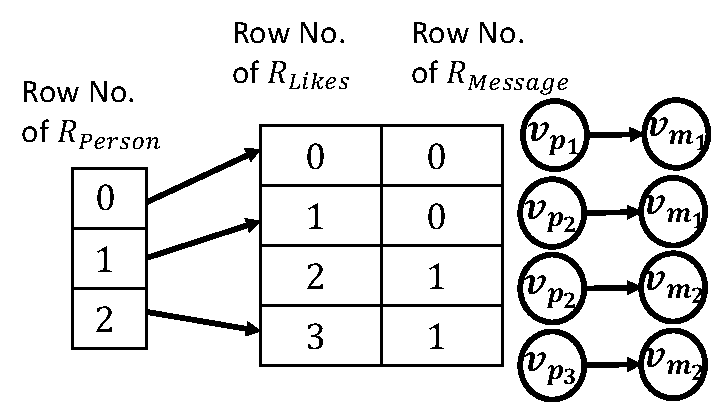
\includegraphics[width=.8\linewidth]{./figures/graph-index-likes.pdf}
    \caption{A graph index on edges labeled ``Likes'' on $G_1$ in \reffig{intro-rgmapping-example}.}
    \label{fig:graph-index}
\end{figure}

\subsection{Graph Index}
\label{sec:graph-index}

In a property graph, the adjacency relationships between vertices and edges are obvious and the adjacent edges of a vertex can be obtained directly.
Moreover, a tuple in a relation corresponds to a vertex or an edge in the property graph according to the \rgmapping.
Therefore, by maintaining the relationships between vertices and edges via indices, the join operator can be markedly accelerated.
This improvement is achieved because for each tuple within a relation, the indices have pre-stored the tuples that are joinable with it.
As a result, it eliminates the necessity to iterate through every tuple of the counterpart relation, thereby enhancing the efficiency of the join process.
As this index structure mimics the adjacency relationship between vertices and edges, it is called a graph index.

Join operators that leverage graph indices are called predefined joins by GrainDB \cite{graindb}.
Specifically, an example of the graph index instantiated in GrainDB is shown in \reffig{graph-index}.
In detail, the graph index is built on edges labeled ``Likes'' in property graph $G_1$ of \reffig{intro-rgmapping-example}(a) and records the adjacency relationships of the vertices labeled ``Person'' and the edges labeled ``Likes''.
That is, according to the \rgmapping, for each tuple $t_p$ in $\relation{Person}$, the tuples in $\relation{Likes}$ that can be joined with $t_p$ can be directly obtained with the graph index and vice versa.

In detail, the graph index consists of two parts as shown in \reffig{graph-index}.
The first part in \reffig{graph-index}(a) is designed for efficiently accessing tuples in $\relation{Person}$ that can be joined with tuples in $\relation{Likes}$.
Specifically, a new column named ``pid\_rowid'' is added to $\relation{Person}$ and the new relation with more columns is called $\grelation{Person}$.
For each tuple $t \in \grelation{Person}$, $t.pid\_rowid$ is the row number of $t_p \in \relation{Person}$, where $t_p.person\_id = t.pid$.
Note that row numbers start from 0.
Take the first tuple in $\grelation{Likes}$ (denoted as $t_l$) as an example.
Because $t_l.pid = p_1$ and the tuple $t_p$ at row number 0 in $\relation{Person}$ satisfies $t_p.person\_id = p_1 = t_l.pid$, we have $t_l.pid\_rowid = 0$.
With this graph index, given a tuple $t$ in $\grelation{Likes}$, the tuple in $\relation{Person}$ that are joinable with $t$ can be retrieved without scanning $\relation{Person}$.

However, given a tuple $t_p$ in $\relation{Person}$, we cannot leverage the graph index in \reffig{graph-index}(a) to directly access tuples in $\grelation{Likes}$ joinable with $t_p$, because it is unknown which rows of $\grelation{Likes}$ contain $pid$ values equal to $t_p.person\_id$.
Therefore, the adjacency list in \reffig{graph-index}(b) is constructed to solve this problem.
To elaborate, the first column contains the row numbers in $\relation{Person}$.
For example, row number 1 represents the second tuple in $\relation{Person}$ with $person\_id = p_2$ (denoted by $t_{p_2}$) and this tuple corresponds to $v_{p_2}$ in $G_1$.
The second column records the row numbers in $\grelation{Likes}$.
With this column, the edges adjacent to a given vertex can be retrieved efficiently.
For example, the edges adjacent to $v_{p_2}$ (i.e., $e_{l_2}$ and $e_{l_3}$ in $G_1$) are stored at row 1 and row 2 of $\grelation{Likes}$.
It means that the second and third tuples in $\grelation{Likes}$ can be joined with $t_{p_2}$.

If the adjacent relationships between vertices labeled ``Message'' and edges labeled ``Likes'' are also recorded in this index, the third column in \reffig{graph-index} is added.
With this column, the neighbors of given vertices can be quickly accessed.
It means that given a tuple $t_p$ in $\relation{Person}$, let $T_{Likes}$ be the set of tuples in $\relation{Likes}$ which can be joined with $t_p$, and then the tuples in $\relation{Message}$ which can be joined with a tuple in $\relation{Likes}$ can be quickly obtained.
For example, the neighbors connected to $v_{p_2}$, connected through edges labeled ``Likes'', include $v_{m_1}$ and $v_{m_2}$, whose corresponding tuples are at row 0 and row 1 in $\relation{Message}$.
This information can be quickly ascertained through the graph index.

\subsection{Physical Implementation of Join and Matching Operators}
\label{sec:join-matching-operator}
In implementing a logical matching plans, the inputs of join operators are two relations, i.e., $R_1 \Join R_2$, where $\theta$ is the join condition.
The join operators can be divided into three categories based on $R_2$.

Firstly, if $R_2$ is not obtained by a matching operator, then the join operator is implemented with
\begin{equation*}
    R_1 \Join R_2.
\end{equation*}

Secondly, if $R_2$ is obtained by a matching operator whose pattern graph is an edge, then the join operator is implemented as an \expandvertex~operator.
Specifically, denote the matching operator by $\matching(\pattern_e)$, where $\pattern_e$ consists of two vertices $u_s, u_t$ and an edge $e$ connecting them.
Let $\lambda^s_e$ and $\lambda^t_e$ be functions that associate tuples in $\relation{\vlabel{(e)}}$ with those in $\relation{\vlabel(u_s)}$ and $\relation{\vlabel(u_t)}$, respectively.
Then, the $\expandvertex(R_1, \pattern_e)$ is implemented with
\begin{equation*}
    R_1 \Join (\relation{\vlabel{(u_s)}} \Join_{\lambda^{s}_{e}} \relation{\vlabel{(e)}} \Join_{\lambda^{t}_{e}} \relation{\vlabel{(u_t)}}).
\end{equation*}
If graph indices have been built on $\relation{\mathcal{L}(e)}$, the joins between $\relation{\mathcal{L}(u_s)}$, $\relation{\mathcal{L}(e)}$, and $\relation{\mathcal{L}(u_t)}$ can be implemented more efficiently by leveraging the graph indices.
Moreover, if there is no need to retain attributes on $e$ and there are no constraints on $e$, graph indices can be applied to get neighbors of $u_s$ directly without scanning $\relation{\mathcal{L}(e)}$.

Thirdly, if $R_2$ is obtained by a matching operator whose pattern graph is a complete star, then the join operator is implemented as an \expandintersect~operator.
Before the \expandintersect~operator is defined, we first propose the $\intersect(alist, rlist)$~operator.
Specifically, the \intersect~operator takes a list of attribute names $alist$ and a list of relations $rlist = \{\relation{1}, \cdots, \relation{m}\}$ as inputs.
Attributes in $alist$ are shared by relations in $rlist$.
Let $t_1, \cdots, t_k$ be tuples in $\relation{1}, \cdots, \relation{m}$, respectively.
These tuples are joined together if and only if they have the same values on attributes in $alist$.


Denote the matching operator by $\matching(\pattern_s)$, where $\pattern_s = (v_r; \mathcal{H})$ and $\mathcal{H} = \{v_1, \cdots, v_k\}, k \geq 2$.
Let $e_1, \cdots, e_k$ be the edges connecting $v_1, \cdots, v_k$ and $v_r$, respectively.
Moreover, we have $\lambda^s_{e_i}$ and $\lambda^t_{e_i}$ mapping tuples from $\relation{\lab(e_i)}$ to $\relation{\lab(v_i)}$, and from $\relation{\lab(e_i)}$ to $\relation{\lab(v_r)}$, respectively.
Then, the $\expandintersect$($\relation{1}$, $\pattern_s$)~operator is implemented as
\begin{equation*}
    \intersect(\{v_r\}, \{\expandvertex(R_1, \pattern_{v_1}), \cdots, \expandvertex(R_1, \pattern_{v_k})\}),
\end{equation*}
where $\pattern_{v_i}$ represents a pattern with an edge connecting $v_i$ and $v_r$.

\begin{example}
    Given the pattern graph $\pattern$ shown in \reffig{intro-rgmapping-example}(b), a possible physical implementation for $\matching(\pattern)$ is as follows:
    \begin{equation*}
        \expandintersect(\expandvertex(\relation{\lab(u_{p_1})}, \pattern_{0}), \pattern_{s}),
    \end{equation*}
    where $\pattern_{0}$ consists of an edge connecting $u_{p_1}$ and $u_{p_2}$, while $\pattern_{s}$ is a complete star with $v_r = u_m$ and $\mathcal{H} = \{u_{p_1}, u_{p_2}\}$.
\end{example}
